% !Mode:: "TeX:UTF-8"
% !TEX program  = xelatex
\documentclass[a4paper]{article}
\usepackage{amsmath}
\usepackage{amssymb}
\usepackage{ctex}
%\usepackage{braket}
\usepackage[european]{circuitikz}
\usepackage{multirow}
\usepackage{float}
\usepackage{geometry}
\geometry{left=2.5cm,right=2.5cm,bottom=2.5cm,top=2.5cm}
\title{模电实验报告5:集成功率放大器}
\author{xy\quad 学号\quad 匡亚明学院}
\date{2019年2月29日}
\begin{document}
\maketitle
\bibliographystyle{unsrt}
%--------main-body------------

\section{实验目的}
\begin{enumerate}
\item 进一步熟悉集成功率放大器的工作原理.
\item 掌握测量集成功率放大器性能的方法.
\end{enumerate}

\section{实验仪器}
双踪示波器、信号发生器、交流毫伏表、数字万用表.

\section{预习内容}
\begin{enumerate}
\item 功率放大器的工作原理.
\item 阅读附录3,分析LM386原理电路在1、8端开路时的电压放大倍数为什么为20.
\item 阅读附录3,试述图(\ref{cd1})中的四个电容的作用.
\end{enumerate}

\section{实验内容}
通常一个实用的放大器包括输入放大器,电压放大器和输出放大器.输入放大器的主要任务是接收传感器输出的小信号,通常要求输入放大器在具有电压放大能力的同时还具有高输入电阻、高抗干扰能力和低噪声.电压放大器的主要任务是不失真地提高输入信号的幅度.输出放大器的主要任务是驱动末级负载.负载是多种多样的,负载电阻的阻值越小,负载越重.有的负载较重,例如,扬声器,电机等.这就要求放大器能输出一定的信号功率,通常称这样的输出放大器为功率放大器.
功率放大器主要任务是在信号不失真或轻度失真的条件下提高输出功率.通常工作在大信号状态下,要求输出功率大、效率高的同时,还要考虑减小非线性失真、功率管的散热、过压过流保护等.静态电流是造成管耗的主要因素,因此在低频功放中主要采用静态工作点低的甲乙类和乙类功率放大器.
实验电路如图(\ref{cd1}).
\begin{figure}[!h]
\centering
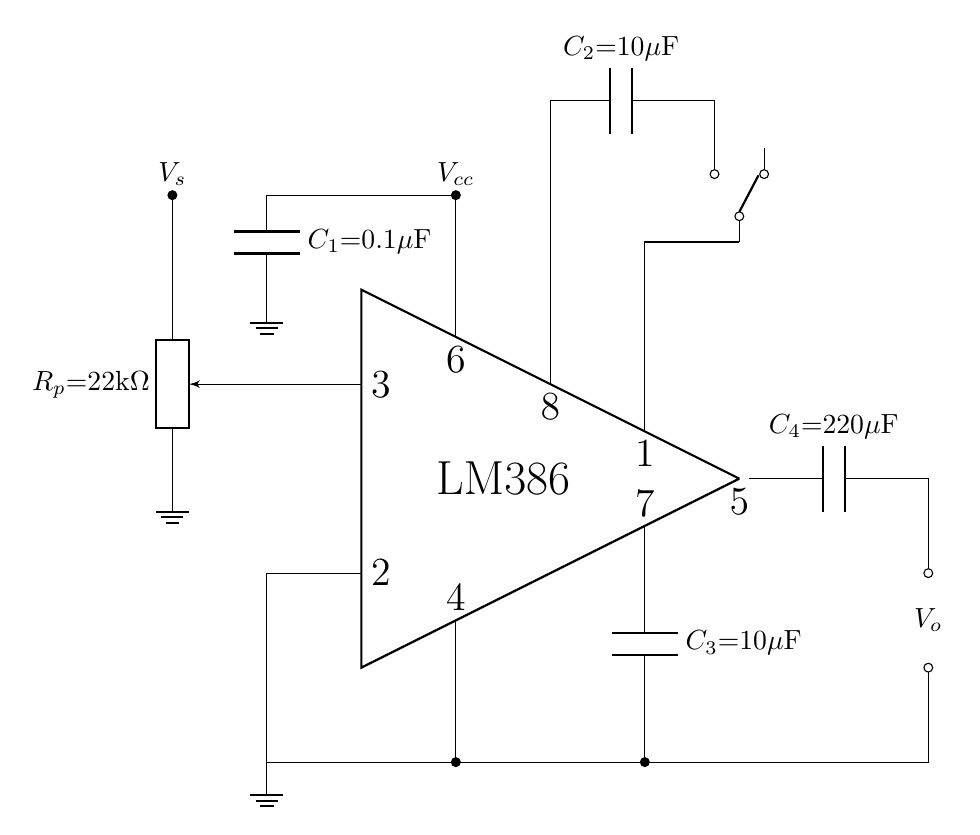
\begin{tikzpicture}[x = 1.2cm, y = 1.2cm]
	\draw[thick] (4,0) -- (0,-2) -- (0,2) -- (4,0);

	\draw[color = black]
	(3,0.5) node[anchor = north](N1){\Large1} 	%1
	(0,-1) node[anchor = west](N2){\Large2}		%2
	(0,1) node[anchor = west](N3){\Large3}		%3
	(1,-1.5) node[anchor = south](N4){\Large4}	%4
	(4,0) node[](N5){} node[anchor = north]{\Large5}		%5
	(1,1.5) node[anchor = north](N6){\Large6}	%6
	(3,-0.5) node[anchor = south](N7){\Large7}	%7
	(2,1) node[anchor = north](N8){\Large8} 	%8

	(4,3) node[spdt, rotate = 90, xscale = 1, yscale = -1](K){}
	(N1) |- (K.in)
	(N8) -- (2,4) to [C, l^=$C_2{=}10\mu\text{F}$] (3.5,4) -| (K.out 2)
	(N6) -- (1,3) node[circ]{} node[anchor = south]{$V_{cc}$} -- (-1,3) to [C, l^= $C_1{=}0.1\mu\text{F}$] (-1,2) node[ground](){}
	(-2,3) node[anchor = south](){$V_s$} to [short, *-] (-2,2) to [pR, l_=$R_p{=}22\text{k}\Omega$, n = pR] (-2,0) node[ground](){}
	(N3) -- (pR.wiper)
	(N2) -| (-1,-3) node[ground](GND){} -- (6,-3) to [short, -o] (6,-2);
	\draw (1,-1.5) to [short, -*] (1,-3);
	\draw (3,-0.5) to [C, l=$C_3{=}10\mu\text{F}$, -*] (3,-3);
	\draw (N5) to [C, l^= $C_4{=}220\mu\text{F}$] (6,0) to [short, -o] (6,-1);
	\draw (6,-1.5) node[]{$V_o$}
		  (1.5,0) node[]{\LARGE LM386};
\end{tikzpicture}\\
\caption{集成功率放大器电路图}\label{cd1}
\end{figure}
\begin{enumerate}
\item 对LM386内部等效电路的分析\\
LM386为单直流电源供电的普通音频功率放大器,常用于袖珍式收音机、磁带放音机,其等效原理示意图如图(\ref{cd2}).
\begin{figure}[!h]
\centering
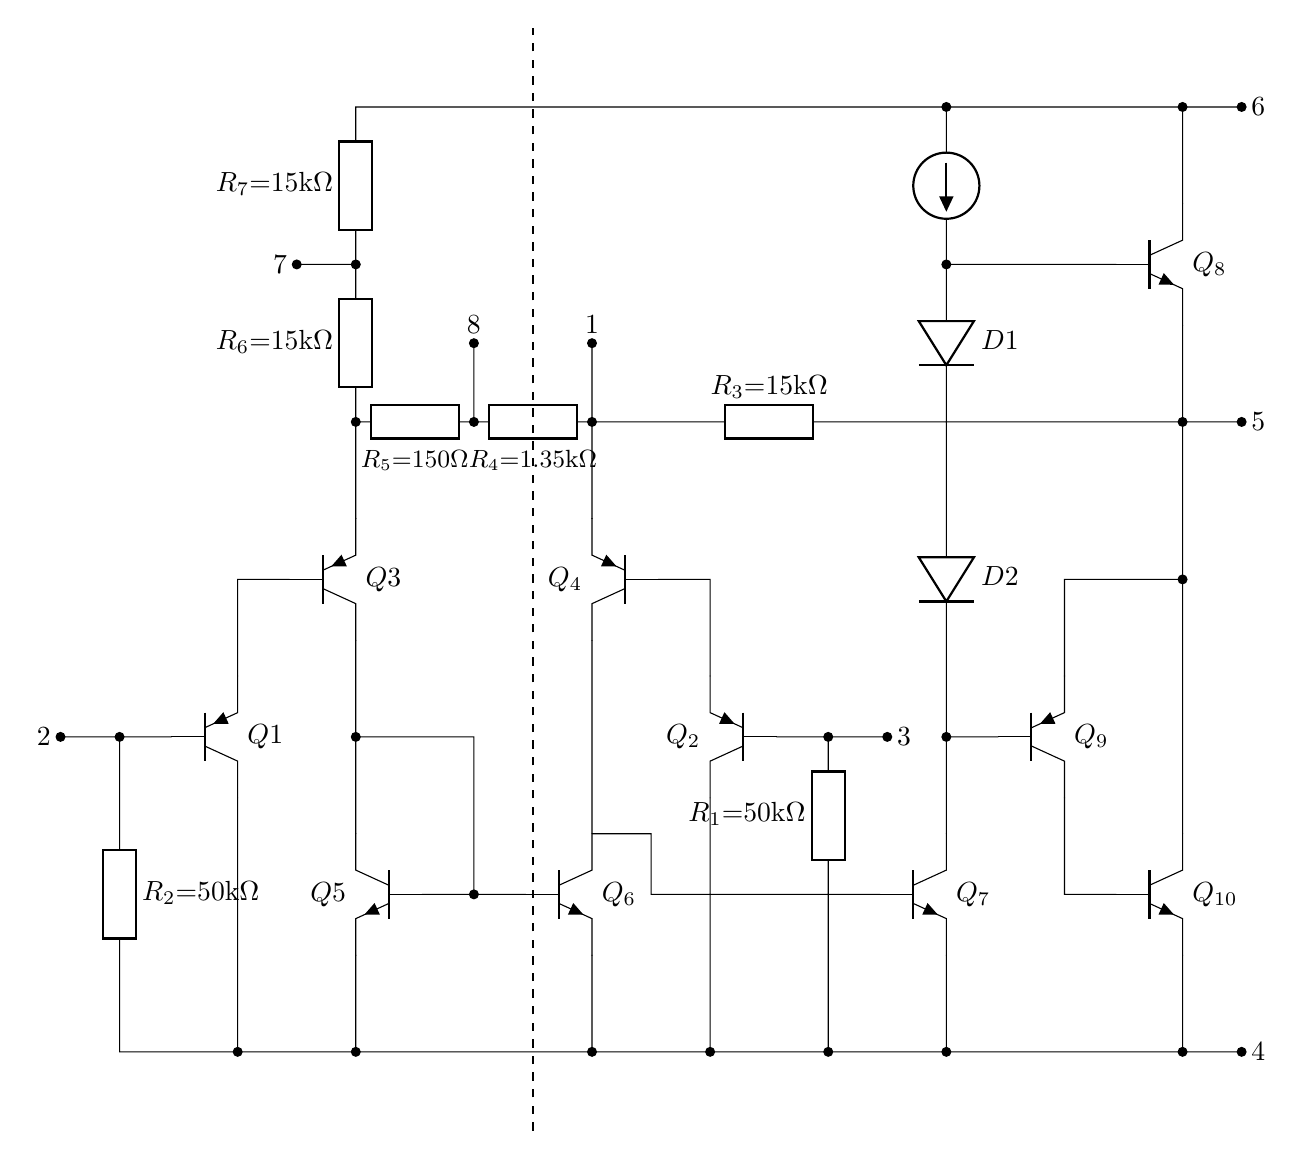
\begin{tikzpicture}[x = 1.5cm, y = 2cm]
	\draw[color = black]

	(1,2) node[pnp](Q1){} node[right]{$Q1$}
	(2,3) node[pnp](Q3){} node[right]{$Q3$}
	(2,1) node[npn, xscale = -1](Q5){} node[left]{$Q5$}
	(4,3) node[pnp, xscale = -1](Q4){} node[left]{$Q_4$}
	(5,2) node[pnp, xscale = -1](Q2){} node[left]{$Q_2$}
	(4,1) node[npn](Q6){} node[right]{$Q_6$}
	(7,1) node[npn](Q7){} node[right]{$Q_7$}
	(9,5) node[npn](Q8){} node[right]{$Q_8$}
	(8,2) node[pnp](Q9){} node[right]{$Q_9$}
	(9,1) node[npn](Q10){} node[right]{$Q_{10}$}

	(-0.5,2) node[left]{2} to [short, *-*] (0,2)
			 to [R = $R_2{=}50\text{k}\Omega$] (0,0)
			 to [short, -*] (1,0)
			 to [short] (Q1.C)
	(0,2) to [short] (Q1.B)
	(Q1.E) |- (Q3.B)
	(Q3.C) to [short, -*] (2,2)
		   to [short] (Q5.C)
	(Q5.E) to [short, -*] (2,0)
		   to [short] (1,0)
	(2,2) -| (3,1)
	(Q3.E) to [short] (2,4)
		   to [R = $R_6{=}15\text{k}\Omega$] (2,5)
		   to [R = $R_7{=}15\text{k}\Omega$, *-] (2,6)
		   to [short] (3,6)
	(Q5.B) to [short, -*] (3,1) -- (Q6.B)
	(2,0) -- (3,0) -- (4,0)
	(2,5) to [short, -*] (1.5,5) node[left]{7}

	(2,4) to [R, l_=\small $R_5{=}150\Omega$, *-] (3,4)
		  to [R, l_=\small $R_4{=}1.35\text{k}\Omega$, -*] (4,4)
		  -- (Q4.E)
	(Q4.C) -- (Q6.C)
	(Q6.E) to [short, -*] (4,0)
		   to [short, -*] (5,0)
		   to [short, -*] (6,0)
		   to [short, -*] (7,0)
		   to [short, -*] (9,0)
		   to [short, -*] (9.5,0) node[right]{4}
	(5,0) -- (Q2.C)
	(Q4.B) -| (Q2.E)
	(Q2.B) to [short, -*] (6,2)
		   to [R, l_= $R_1{=}50\text{k}\Omega$] (6,1) -- (6,0)
	(Q6.C) -| (4.5,1) -- (Q7.B)
	(Q7.E) -- (7,0)
	(Q7.C) -- (7,2) to [short, *-] (Q9.B)
	(6,2) to [short, -*] (6.5,2) node[right]{3}
	(4,4) to [R = $R_3{=}15\text{k}\Omega$] (7,4) -- (9,4)
	(Q8.E) to [short, -*] (9,4)
		   to [short, -*] (9,3) -| (Q9.E)
	(9,3) -- (Q10.C)
	(Q9.C) |- (Q10.B)
	(Q10.E) -- (9,0)
	(3,4) to [short, *-*] (3,4.5) node[anchor = south]{8}
	(4,4) to [short, -*] (4,4.5) node[anchor = south]{1}
	(3,6) -- (7,6)
		  to [american current source, *-*] (7,5)
		  to [D,  l= $D1$] (7,4)
		  to [D,  l= $D2$] (7,2)
	(7,5) -- (Q8.B)
	(7,6) -| (Q8.C)
	(9,6) to [short, *-*] (9.5,6) node[right]{6}
	(9,4) to [short, -*] (9.5,4) node[right]{5};

	\draw[dashed] (3.5, -0.5) -- (3.5, 6.5)
	;
\end{tikzpicture}
\caption{LM386等效原理示意图}\label{cd2}
\end{figure}
等效原理示意图并不是真实的电路图,而是为了使用者了解集成电路的原理,从而正确地设计外电路,而画出的等效原理电路.

LM386由输入级、中间级和输出级三部分组成.三极管$Q_1$~$Q_4$构成复合管差动输入级,$Q_5$、$Q_6$构成的镜像电流源作为差动放大器的集电极有源负载.输入级的单端输出信号由$Q_4$的集电极传送至由$Q_7$组成的中间级,该级是以恒流源为集电极负载的共射极放大器.$Q_8$、$Q_9$、$Q_{10}$和$D_1$、$D_2$组成通常的甲乙类互补对称输出级.$Q_9$、$Q_{10}$等效于一个PNP型管,这是考虑到集成电路中PNP管的电流放大系数较低,故用复合管提高电流放大系数.$D_1$、$D_2$为输出级提供适当的偏压,以克服交越失真,保证电路工作在甲乙类工作状态.

差动输入级的静态工作电流,分别由输出端经$R_3$和电源正端通过电阻$R_7$和$R_6$来供给.“6”端为直流偏置电压$V_{CC}$,“5”端为输出端,其静态电压为$V_{CC}/2$,$Q_3$发射极静态电流与$Q_4$发射极静态电流相等.差动输入级电路左右对称.所以,差动输入级有较高的CMRR.

通常,功率放大器的信号源内阻并不大,所以在差动输入级的两个输入端对地接了50k$\Omega$电阻,以减小输入电阻,这对输入信号的衰减可忽略,但可减少高内阻共模信号的接收,减少输出端的共模干扰.输入级和中间级因为用恒流源做集电极负载,所以具有很高的电压放大倍数,因此可引入级间负反馈,以大大改善电路的性能.反馈支路由$R_3$和$R_4$、$R_5$组成.若将差动输入级用一对称轴(虚线)划分两半,则阻值R=($R_4$+$R_5$)/2=750$\Omega$处为等效交流地电位点.用瞬时极性法可以判断,所引入的是电压串联负反馈,其反馈系数为:$F_v$=R/($R_3$+R).这样就能维持电压放大倍数恒定.输入信号可以从两端输入,也可以从单端输入.若如本实验电路,“3”端为输入,“4”端接地,则LM386的电压放大关系可等效为图(\ref{cd3})
\begin{figure}[!h]
\centering
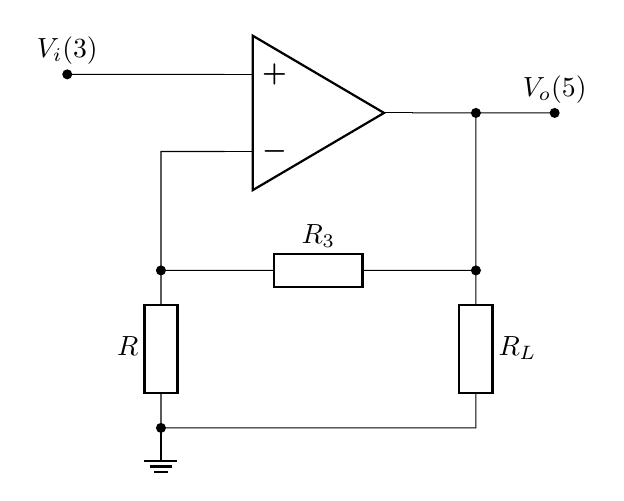
\begin{tikzpicture}[x = 2cm, y = 2cm]
	\draw
	(0,0) node[op amp, yscale = -1](AMP){}
	(AMP.out) -- (1,0) -- (1,-1) to [R = $R_L$] (1,-2) -- (-1,-2) node[ground]{} node[circ]{} to [R = $R$] (-1,-1) |- (AMP.-)
	(-1,-1) to [R = $R_3$, *-*] (1,-1)
	(AMP.+) --++ (-1,0) node[circ]{} node[anchor = south]{$V_i(3)$}
	(1,0) to [short, *-*] (1.5,0) node[anchor = south]{$V_o(5)$}
	;
\end{tikzpicture}
\caption{LM386等效放大电路}\label{cd3}
\end{figure}
,为同相输入电压放大器.若“1”、“8”端交流开路,其交流放大倍数约为
\begin{equation}
A_V \approx \cfrac{1}{F_V} = 1+\cfrac{R_3}{R} = 21\label{eq1}
\end{equation}
若“1”、“8”端接10$\mu$F电容,可近似“1”、“8”观短路,其电压放大倍数约为
\begin{equation}
A_V = \cfrac{1}{F_V} = 1+\cfrac{R_2}{R_5/2} = 201
\end{equation}
对图(\ref{cd1})中的电容$C_3$的作用试述如下.若不接$C_3$,对于交流信号,在图(\ref{cd2})中,“6”端接$V_{CC}$,$V_{CC}$内阻通常小于1$\Omega$,因此可近似为交流信号从Q3发射极经$R_6$、$R_7$两个15k$\Omega$电阻到地;输出负载通常为几$\Omega$至几十$\Omega$,因此可近为交流信号从$Q_4$发射极经$R_3$一个15k$\Omega$电阻到地;所以差动输入级对于交流信号是严重不平衡的.接$C_3$后,对于直流没有作用,对于交流使$Q_3$、$Q_4$到地的电阻值近似相等,从而使差动输入级能正常放大差模信号和抑制共模干扰.

\item 实验内容\\
本实验电路用的是LM386-2,其最大输出功率为0.5W.实验中“1”、“8”端开路,LM386的电压放大倍数约为20倍,负载为8$\Omega$的喇叭,所以输入电压有效值不能超过100mV,为减少损坏,加在图(\ref{cd1})所示电位器$R_p$上端的电压不得超过90mV.
\begin{enumerate}
\item 取$V_{CC}$=12V,有效值$v_i$=50mV,开关K打开,不接负载,改变频率,测量功放的幅频特性,绘制幅频特性曲线.
\item 接负载$R_L$=8$\Omega$的喇叭,重复(1).将幅频特性曲线与(1)的绘制在同一张图上.
\item $V_{CC}$=12V,f=1kHz,开关K打开,不接负载,改变输入电压(请特别注意,输入不得超过90mV!!否则有可能损坏LM386!!),测量功放的输入-输出特性曲线.
建议按表(\ref{tableIO})要求测量.

\item 接负载$R_L$=8$\Omega$的喇叭,重复(3).将输入-输出特性曲线与(3)的绘制在同一张图上.建议按表(\ref{tableIO})要求测量.
\item 取$V_{CC}$=5V、9V、12V,f=1kHz,有效值$v_i$=50mV,测量并估算功放的输出交流功率P、直流电源消耗功率$P_V$(忽略LM386中电压放大电路的功耗,仅计及功率放大电路的功耗)和效率$\eta$.
对于正弦信号,在正半周$Q_8$导通,$Q_9$、$Q_{10}$组成的复合管截止,$Q_8$集电极上的功耗为
\begin{eqnarray}
P_{Q_8}
 &=& \frac{1}{2\pi}\int^{\pi}_{0}\left(\frac{V_{CC}}{2} - v_o\right)\frac{v_o}{R_L}\text{d}(\omega t)\\
 &=& \frac{1}{2\pi}\int^{\pi}_{0}\left(\frac{V_{CC}}{2} - v_{om}\sin(\omega t)\right)\frac{v_{om}\sin(\omega t)}{R_L}\text{d}(\omega t)\\
 &=& \frac{1}{2\pi}\int^{\pi}_{0}\left[\frac{V_{CC}v_{om}}{2R_L}\sin(\omega t) - \frac{v_{om}^2}{RL}\sin^2(\omega t)\right]\text{d}(\omega t)\\
 &=& \cfrac{1}{R_L}\left(\cfrac{V_{CC}v_{om}}{2\pi} - \cfrac{v_{om}^2}{4}\right)
\end{eqnarray}
在负半周$Q_8$截止,$Q_9$、$Q_{10}$组成的复合管导通,复合管等效集电极上的功耗P$Q_9$、10$\approx$P$Q_8$.负载在一个周期中得到的功率为
\begin{equation}
P_o = \cfrac{v^2_{om}}{2R_L} = \cfrac{v_{rms}^2}{R_L}
\end{equation}
其中,$v_{om}$为正弦信号的幅值,$v_{rms}$为正弦信号的有效值.所以直流电源的功耗为
\begin{equation}
P_V \approx 2P_{QS}+P_o = \cfrac{V_{CC}v_{om}}{\pi R_L} = \cfrac{V_{CC}\sqrt{2}v_{orms}}{\pi R_L}
\end{equation}
效率近似为
\begin{equation}
\eta = \cfrac{P_o}{P_V} = \cfrac{\pi v_{om}}{2V_{CC}} = \cfrac{\pi v_{orms}}{\sqrt{2}V_{CC}}\label{eta}
\end{equation}
\end{enumerate}
\end{enumerate}

\section{实验数据}
\begin{enumerate}
\item 幅频响应\\
幅频响应的数据如下,注意两次的$v_s$不同.
\begin{enumerate}
\item 空载\\
此时$v_i$ = 50.051mV,$v_o$ = 1.0776V, 得到$v_{o'}$ = 0.7619V.通频带为:\\
$f_\text{L}$ = 1Hz, $f_\text{H}$ = 469kHz
\item 有载\\
此时$v_i$ = 30.624mV,$v_o$ = 611.994mV, 得到$v_{o'}$ = 432.745mV.通频带为:\\
$f_\text{L}$ = 114Hz, $f_\text{H}$ = 741kHz
\end{enumerate}
因为仅仅测量了三个数据点,不足以画出真实的幅频特性曲线,因此在最后的原始数据胖手工绘制草图.
\item 输入输出曲线\\
输入输出特性的数据如表(\ref{tableIO}):
\begin{table}[!h]
\centering
\caption{输入输出特性曲线}
\label{tableIO}
\begin{tabular}{|c|c|c|c|c|c|c|c|c|c|}
\hline
\multirow{2}{*}{空载} & $V_i$(mV) & 10.340  & 20.027  & 30.712  & 40.666  & 50.370   & 60.435   & 70.762   & 79.784   \\ \cline{2-10} 
                    & $V_o$(mV) & 214.341 & 427.522 & 659.351 & 875.732 & 1085.275 & 1302.617 & 1526.101 & 1720.312 \\ \hline
\multirow{2}{*}{有载} & $V_i$(mV) & 10.108  & 20.059  & 30.025  & 40.225  & 50.295   & 60.245   & 70.160   & 79.862   \\ \cline{2-10} 
                    & $V_o$(mV) & 191.050 & 394.102 & 599.005 & 801.348 & 1004.783 & 1204.977 & 1404.835 & 1599.628 \\ \hline
\end{tabular}
\end{table}

根据表(\ref{tableIO}),画出输入输出特性曲线,如图(\ref{figIO}):
\begin{figure}[!h]
\centering
\includegraphics[width=12cm]{fig/IO.pdf}\\
\caption{输入输出特性曲线}\label{figIO}
\end{figure}
\item 效率\\
在$v_i$=50.212mV下,实验测得$v_{orms}$=1006.269mV,算得效率为:
\begin{equation}
\eta = \cfrac{\pi v_{orms}}{\sqrt{2}V_{CC}} \approx 18.63\%
\end{equation}
\end{enumerate}

\section{误差分析}
\begin{enumerate}
\item 低频截止频率\\
在测量空载低频截止频率时,我们发现测量值已经小于6Hz,并且万用表示数波动范围非常大.因此空载低频截止频率的误差较大.
\item 谐波失真\\
在网站上的视频中我们注意到,在示波器上的波形已经肉眼可见明显的非线性谐波失真,说明该实验中非线性谐波失真是很严重的.
\end{enumerate}

\section{思考题}
\begin{enumerate}
\item \textbf{试画出进一步简化的、说明LM386的电压放大倍数的示意图.}\\
进一步简化的LM386等效电路图如图(\ref{LM386s})所示:
\begin{figure}[!h]
\centering
\begin{tikzpicture}[x = 3cm, y = 2cm]
\draw (0,0) node[ground](GND){} to [short, *-*] (3,0);
\draw (0,2) to [R, l =\large $r_i$, o-*] (1,2) to [R, l = $R$, -*] (1,0);
\draw (1,2) to [R, l = $R_3$, -*] (2,2) to [R, l = $R_L$, -*] (2,0);
\draw (2,2) to [short, -*] (3,2) to [R, l =\large $r_o$] (3,1);
\draw (3,1) -- (3,0.8) -- (3.1,0.5) -- (3,0.2) -- (2.9,0.5) -- (3,0.8);
\draw (3,0) -- (3,0.2);
\draw (3,2) to [short, -o] (3.5,2);
\draw (0,2) node[anchor=east]{\large $v_i$}
      (3.5,2) node[anchor=west]{\large $v_o$}
      (3.75,0.5) node[anchor=east]{$A_V(v_i - v_1)$}
      (1,2) node[anchor=south]{\large $v_1$}
      (2,2) node[anchor=south]{\large $v_2$}
;
\end{tikzpicture}
\caption{LM386简化等效电路图}\label{LM386s}
\end{figure}

通过计算$v_1$和$v_2$处的电压关系,可以近似得到如式(\ref{eq1})所示的电压放大倍数.
\item \textbf{试述图(\ref{cd1})中的四个电容的作用,以及改变电容参数对整个电路的性能的影响.}\\
在实验中只用了三个电容:$C_1$、$C_3$、$C_4$,它们的作用基本都是滤波,细节分别为:
\begin{enumerate}
\item $C_1$直流电压耦合,起“水塘”作用,减小直流电压中可能存在的交流成分对电路静态的影响.
\item $C_3$改变共模抑制比.\\
如前文所述:若不接$C_3$,对于交流信号,在图(\ref{cd2})中,“6”端接$V_{CC}$,$V_{CC}$内阻通常小于1$\Omega$,因此可近似为交流信号从Q3发射极经$R_6$、$R_7$两个15k$\Omega$电阻到地;输出负载通常为几$\Omega$至几十$\Omega$,因此可近为交流信号从$Q_4$发射极经$R_3$一个15k$\Omega$电阻到地;所以差动输入级对于交流信号是严重不平衡的.接$C_3$后,对于直流没有作用,对于交流使$Q_3$、$Q_4$到地的电阻值近似相等,从而使差动输入级能正常放大差模信号和抑制共模干扰.
\item $C_4$取交隔直,起负电源作用.
\end{enumerate}
改变这些电容的参数会影响电路的交直流性能,但具体影响不清楚.
\item \textbf{试述负载对功放性能的影响.}\\
加上负载后,集成功率放大器的输出电压略有减小,但是相比其绝对值并不算大,因此可认为对性能没有太大影响.
\item \textbf{试述电源电压对对功放性能的影响.若要求改善功放的输入-输出特性应提高还是降低电源电压?}\\
根据式(\ref{eta})可知,在输入输出电压不变的情况下,效率仅与$V_{CC}$有关,$V_{CC}$越小,效率越高.另外,直流电压越低,输入输出曲线的线性越好.要改善放大器的输入输出特性,应该降低电源电压.
\end{enumerate}

\nocite{jiaocai}
%--------bib------------------
\bibliography{ref}
\end{document}